\documentclass[10pt]{article}

\usepackage{amsmath,amssymb,amsthm}
\usepackage{fancyhdr,url,hyperref}
\usepackage{graphicx,xspace}
\usepackage{tikz}
\usetikzlibrary{shapes,arrows,decorations.pathmorphing,backgrounds,positioning,fit,through}

\oddsidemargin 0in  %0.5in
\topmargin     0in
\leftmargin    0in
\rightmargin   0in
\textheight    9in
\textwidth     6in %6in
%\headheight    0in
%\headsep       0in
%\footskip      0.5in

\newtheorem{thm}{Theorem}
\newtheorem{cor}[thm]{Corollary}
\newtheorem{obs}{Observation}
\newtheorem{lemma}{Lemma}
\newtheorem{claim}{Claim}
\newtheorem{definition}{Definition}
\newtheorem{question}{Question}
\newtheorem{answer}{Answer}
\newtheorem{problem}{Problem}
\newtheorem{solution}{Solution}
\newtheorem{conjecture}{Conjecture}

\pagestyle{fancy}

\newcommand{\shortans}{\vspace{1in}}
\newcommand{\mediumans}{\vspace{1.5in}}
\newcommand{\longans}{\vspace{2in}}

\lhead{\textsc{Prof. McNamara}}
\chead{\textsc{SDS/MTH 291: Lecture notes}}
\lfoot{}
\cfoot{}
%\cfoot{\thepage}
\rfoot{}
\renewcommand{\headrulewidth}{0.2pt}
\renewcommand{\footrulewidth}{0.0pt}

\newcommand{\ans}{\vspace{0.25in}}
\newcommand{\R}{{\sf R}\xspace}
\newcommand{\cmd}[1]{\texttt{#1}}
\DeclareMathOperator{\Ex}{\mathbb{E}}
\DeclareMathOperator{\Var}{\text{Var}}

\rhead{\textsc{October 25, 2016}}

\usepackage{Sweave}
\begin{document}
\Sconcordance{concordance:11_interactionplots.tex:11_interactionplots.Rnw:%
1 53 1 1 0 35 1 1 2 1 0 1 1 3 0 1 2 14 1 1 3 2 0 1 5 3 0 2 1 1 4 2 0 1 %
4 2 0 1 3 1 0 1 2 1 1 1 7 5 0 1 6 4 0 1 3 1 0 1 5 3 0 1 5 3 0 1 2 1 1 1 %
4 2 0 1 3 1 0 1 6 4 0 1 3 1 0 1 7 5 0 1 4 2 0 1 1 1 2 1 0 1 3 1 0 1 14 %
12 0 1 4 2 0 1 3 2 0 1 1 1 3 2 0 1 1 1 3 2 0 1 4 3 0 1 3 2 0 1 1 1 3 2 %
0 1 1 1 3 2 0 1 2 4 0 1 2 2 1}


\paragraph{Agenda}
\begin{enumerate}
  \itemsep0em
  \item Interaction plots
  \item Regression summary lab
  % \item Added Variable Plots
  % \item Model Selection
\end{enumerate}


\paragraph{Interaction plots}
A common way to visualize the interaction between two categorical variables is with an interaction plot. 

\begin{figure}[htbp]
\begin{center}
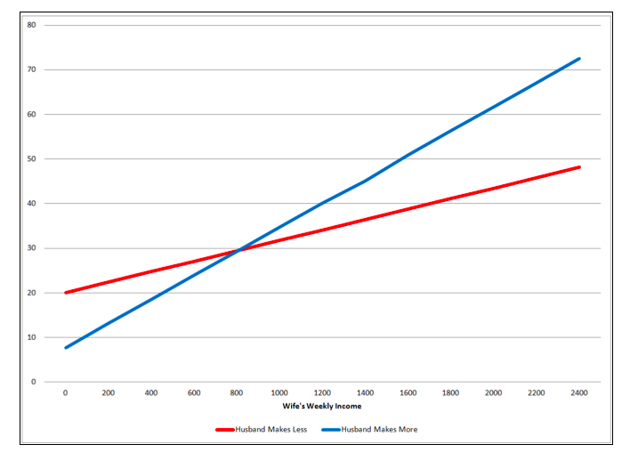
\includegraphics[width=0.7\textwidth]{Atlantic_Chores.png}
\caption{Figure from the Atlantic article, ``Emasculated Men Refuse to Do Chores--Except Cooking.'' \label{atlantic}}
\end{center}
\end{figure}

As an example, consider Figure \ref{atlantic}, from \url{https://www.theatlantic.com/health/archive/2016/10/the-only-chore-men-will-do-is-cook/505067/}


\begin{enumerate}
  \itemsep1in
  \item How can we interpret this plot?
  \item What would the R code associated with this model look like?
  \item What would you expect the fitted coefficients to be like on the  model?
  \shortans
\end{enumerate}

For another example, lets think back to the education data we keep considering

\begin{Schunk}
\begin{Sinput}
> require(openintro)
> with(hsb2, interaction.plot(ses, gender, math))
\end{Sinput}
\end{Schunk}

\begin{enumerate}
  \itemsep1in
  \item How can we interpret this plot?
  \item What would the R code associated with this model look like?
  \item What would you expect the fitted coefficients to be like on the  model?
  \shortans
\end{enumerate}

\clearpage

\clearpage

\paragraph{Regression summary lab} Finally, let's do the regression summary lab

\begin{Schunk}
\begin{Sinput}
> myCars <- vehicles %>%
+   filter(year == 2000 & cyl == 4)
> xyplot(hwy ~ displ, data=myCars, 
+        main="Fuel Economy", alpha=0.5, cex=2, pch=19, 
+        xlab="Engine Size (cubic centimeters)",
+        ylab="Fuel Economy (miles per gallon)")
> m1 <- lm(hwy ~ displ, data=myCars)
> summary(m1)
> regdata <- myCars %>% 
+   mutate(xdif = displ - mean(displ), 
+          ydif = hwy - mean(hwy))
> regdata <- regdata %>% 
+   summarize(SXX = sum(xdif^2), 
+             SXY = sum(xdif*ydif))
> regdata <- regdata %>% 
+   mutate(beta1=SXY/SXX)
> regdata
> coef(m1)["displ"]
> myCars %>% 
+   mutate(xdif = displ - mean(displ), 
+          ydif = hwy - mean(hwy)) %>% 
+   summarize(SXX = sum(xdif^2), 
+             SXY = sum(xdif*ydif),
+             beta1=SXY/SXX) 
> myCars %>% 
+   summarize(n=n(),
+             SXX = var(displ) * (n-1),
+             SXY = cov(hwy,displ) * (n-1),
+             beta1 = SXY/SXX)
> myCars %>% 
+   summarize(beta1 = cor(hwy, displ) * (sd(hwy) / sd(displ)))
> regdata <- myCars %>% 
+   summarize(beta1 = cor(hwy, displ) * (sd(hwy) / sd(displ)),
+             meanX = mean(displ),
+             meanY = mean(hwy))
> # Estimate the intercept, using the fact that the means
> # define a point on the regression line
> regdata %>% 
+   mutate(beta0 = meanY - beta1 * meanX)
> predict(m1, newdata=data.frame(displ=mean(~displ, data=myCars)))
> mean(~hwy, data=myCars)
> # We're going to need differences from the mean down the line, so lets start by computing them
> assessdata <- myCars %>% 
+   mutate(ydif = (hwy - mean(hwy)))
> assessdata <- assessdata %>% 
+   mutate(fitted = fitted(m1))
> assessdata <- assessdata %>%
+   summarize(n = n(),
+             SST = sum(ydif^2),
+             SSE = sum((fitted - hwy)^2),
+             SSM = sum((fitted - mean(hwy))^2))
> assessdata %>% 
+   mutate(SSE + SSM)
> myCars %>% 
+   mutate(ydif = (hwy - mean(hwy)),
+          fitted = fitted(m1))  %>%
+   summarize(SST = sum(ydif^2),
+             SSE = sum((fitted - hwy)^2),
+             SSM = sum((fitted - mean(hwy))^2))
> # Coefficient of determination
> assessdata <- assessdata %>% 
+   mutate(rsq = 1 - SSE / SST)
> rsquared(m1)
> # p is the number of explanatory variables
> p <- 1
> assessdata <- assessdata %>%
+   mutate(adjrsq = 1 - (SSE / (n-1-p)) / (SST / (n-1)))
> testdata <- myCars %>% 
+    mutate(ydif = (hwy - mean(hwy)),
+          fitted = fitted(m1)) %>%
+   summarize(n=n(),
+             meanX = mean(displ),
+             meanY = mean(hwy),
+             SXX = var(displ) * (n-1),
+             SXY = cov(hwy,displ) * (n-1),
+             beta1 = SXY/SXX,
+             beta0 = meanY - beta1 * meanX,
+             SST = sum(ydif^2),
+             SSE = sum((fitted - hwy)^2),
+             SSM = sum((fitted - mean(hwy))^2))
> # Residual Standard error
> testdata <- testdata %>% 
+   mutate(RSE = sqrt(SSE / (n-2)))
> # Standard error 
> testdata <- testdata %>%
+   mutate(SE1 = RSE / sqrt(SXX))
> testdata %>% glimpse()
> # t-statistic
> testdata <- testdata %>%
+   mutate(t1 = beta1 / SE1)
> testdata %>% glimpse()
> # p-value
> testdata %>%
+   summarize(p = 2 * pt(abs(t1), df=(n-2), lower.tail = FALSE))
> # Compute statistics for the intercept
> # Standard error 
> testdata <- testdata %>%
+   mutate(SE0 = RSE * sqrt((1/n) + (meanX)^2 / SXX))
> # t-statistic
> testdata <- testdata %>%
+   mutate(t0 = beta0 / SE0)
> testdata %>% glimpse()
> # p-value
> testdata %>%
+   summarise(p = 2 * pt(abs(t0), df=(n-2), lower.tail = FALSE))
> anova(m1)
> # F-statistic
> testdata <- testdata %>%
+   mutate(F = (SSM / p) / (SSE / (n-1 - p)))
> testdata %>%
+   summarize(p = pf(F, df1 = p, df2 = n-1 - p, lower.tail=FALSE))
\end{Sinput}
\end{Schunk}

\end{document}

